
\chapter{Resolvendo o Sistema Matriz-vetor}
\section{Tri-diagonalidade da Matriz}

Vimos que, pela escolha que funções da base, grande parte dos termos da nossa matriz $\mathcal{K}$ zeram.

Veja que temos a definição de $\varphi_i(x)$ como:

\[\varphi_i(x) = \begin{cases}
  \dfrac{x - x_{i-1}}{h}, &\forall x \in [x_{i-1}, x_i] \\
  \dfrac{x_{i+1} - x}{h}, &\forall x \in [x_{i}, x_{i+1}] \\
  0 , &\forall x \notin [x_{i-1}, x_{i+1}]
\end{cases}\]

Além disso, temos como definição da matriz $\mathcal{K}$:

\[
  \begin{pmatrix}
    K_{1,1} & ... & K_{1,j} & ... & K_{1,m} \\
    \vdots & \ddots & \vdots & \ddots & \vdots \\
    K_{i,1} & ... & K_{i,j} & ... & K_{i,m} \\
    \vdots & \ddots & \vdots & \ddots & \vdots \\
    K_{m,1} & ... & K_{m,j} & ... & K_{m,m}
  \end{pmatrix},\quad i, j \in \{1, \dots, m\}
\]

sendo:

\[K_{i,j} = \alpha \int_{0}^{1} \varphi_{xi}(x) \varphi_{xj}(x)dx + \beta \int_{0}^{1} \varphi_i(x) \varphi_j(x)dx + \gamma \int_{0}^{1} \varphi_i(x) \varphi_{xj}(x)dx \]

Mas veja que $\varphi_i \varphi_j = 0$ quando $|i - j| > 1$, então temos que $\mathcal{K}$ é uma matriz esparsa tal que:

\[
  \mathcal{K} =
  \begin{pmatrix}
    K_{1,1} & K_{1,2} & 0       & 0 & 0 \\
    K_{2,1} & K_{2,2} & K_{2,3} & 0 & 0 \\
    0       & K_{3,2} & K_{3,3} & \ddots & 0   \\
    0  & 0  & \ddots  & \ddots & K_{m-1,m} \\
    0  & 0  &  0      & K_{m,m-1} & K_{m,m}
  \end{pmatrix}
\]

Sendo assim, temos que resolver um sistema $\mathcal{K}\mathcal{C} = \mathcal{F}$ para $\mathcal{C}$ sendo $\mathcal{K}$ uma matriz tri-diagonal.


\section{Métodos Iterativos}


Podemos utilizar métodos iterativos semelhantes ao método do Ponto Fixo para resolver sistemas lineares se tivermos a garantia de que os autovalores da matriz são todos menores do que 1 visto que, dessa forma, o erro do método convergirá para $0$ conforme provamos em \cite{notas-cocada}. Para a forma da matriz $\mathcal{K}$ específica desse problema, temos que os seus autovalores são menores do que 1 e, consequentemente, esses métodos podem ser utilizados.

Dessa forma, decidimos realizar um teste de performance ao computar o tempo gasto pelo \texttt{contra barra} da linguagem na qual implementamos o sistema dos Elementos Finitos (Julia) e outros métodos que implementamos.

Primeiramente, estamos realizando uma análise de convergência do erro para garantirmos que todos os métodos estão, de fato, dando o mesmo resultado numérico.

\begin{minipage}{0.3\textwidth}
  \begin{figure}[H]
    \centering
    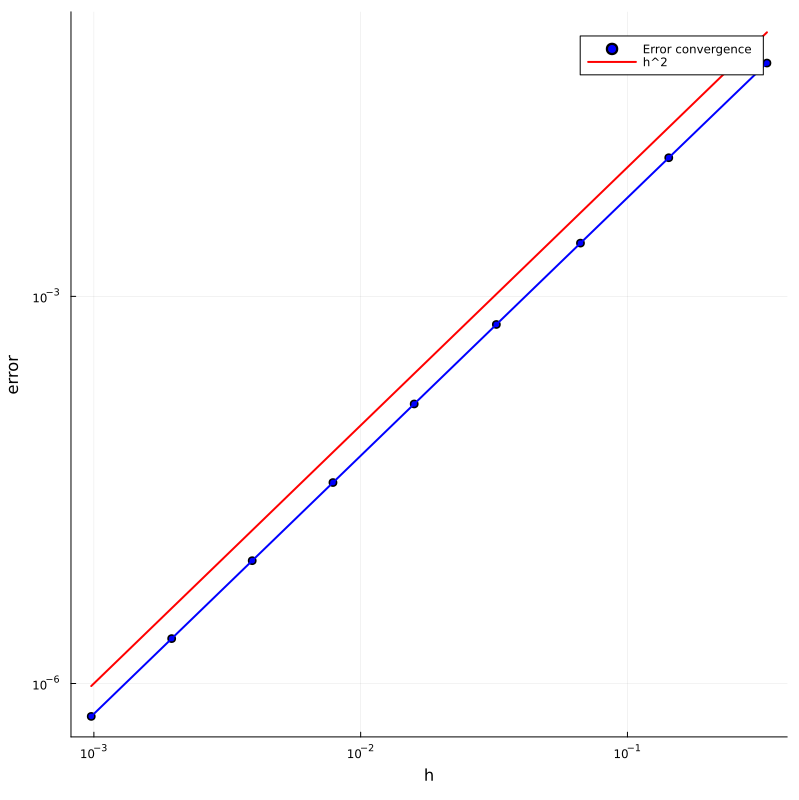
\includegraphics[width=0.85\linewidth]{errors-convergence-Julia backslash.png}
    \caption{Convergência do Erro do \texttt{contra barra} do Julia.}
  \end{figure}
\end{minipage}
\hfill
\begin{minipage}{0.3\textwidth}
  \begin{figure}[H]
    \centering
    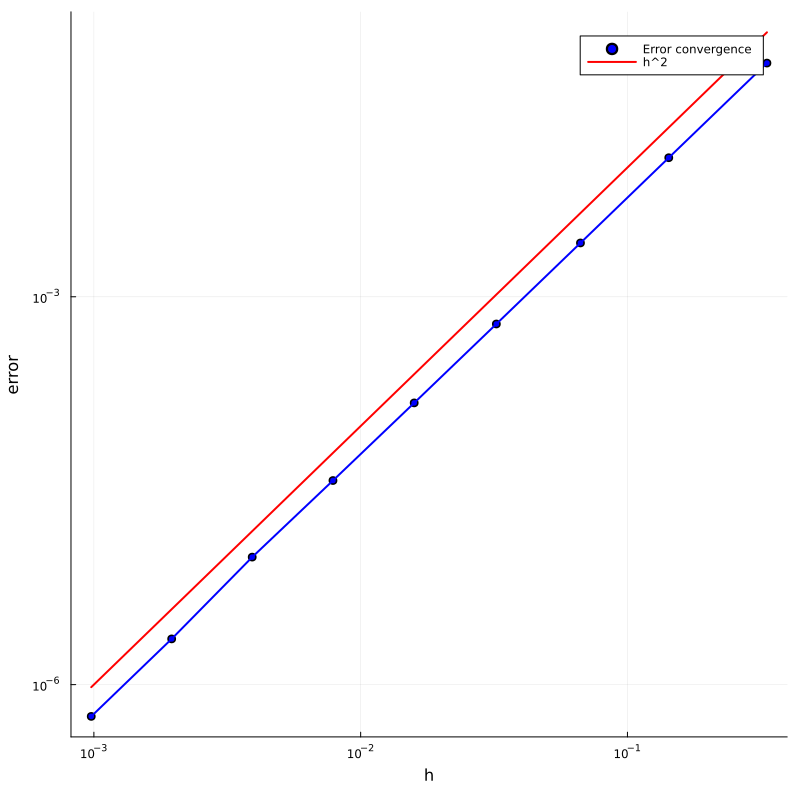
\includegraphics[width=0.85\linewidth]{errors-convergence-Gauss Jacobi.png}
    \caption{Convergência do Erro do Gauss Jacobi.}
  \end{figure}
\end{minipage}
\hfill
\begin{minipage}{0.3\textwidth}
  \begin{figure}[H]
    \centering
    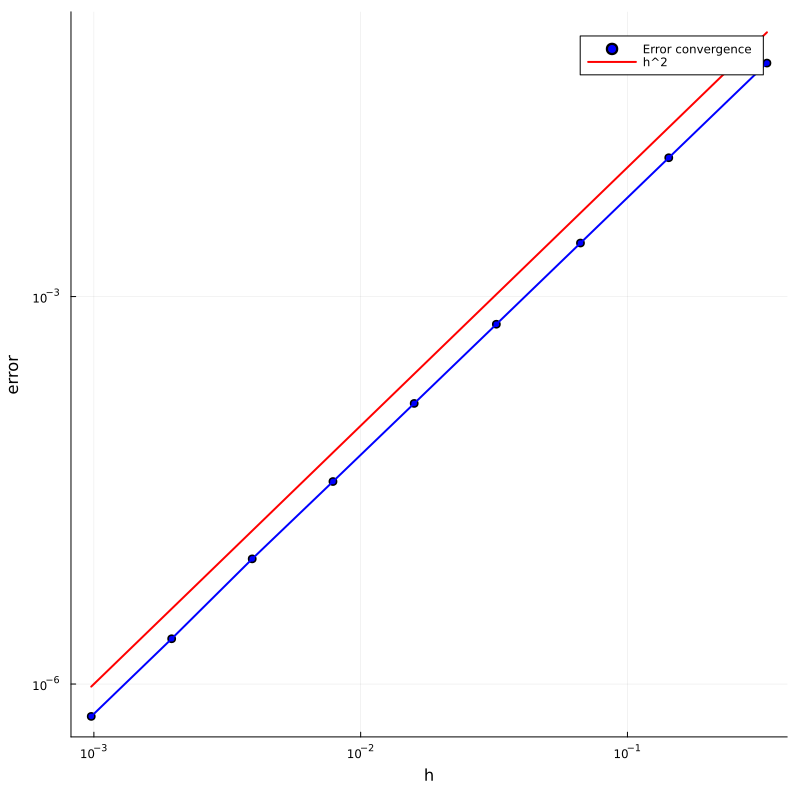
\includegraphics[width=0.85\linewidth]{errors-convergence-Gauss Seidel.png}
    \caption{Convergência do Erro do Gauss Seidel.}
  \end{figure}
\end{minipage}

\begin{minipage}{0.45\textwidth}
  \begin{figure}[H]
    \centering
    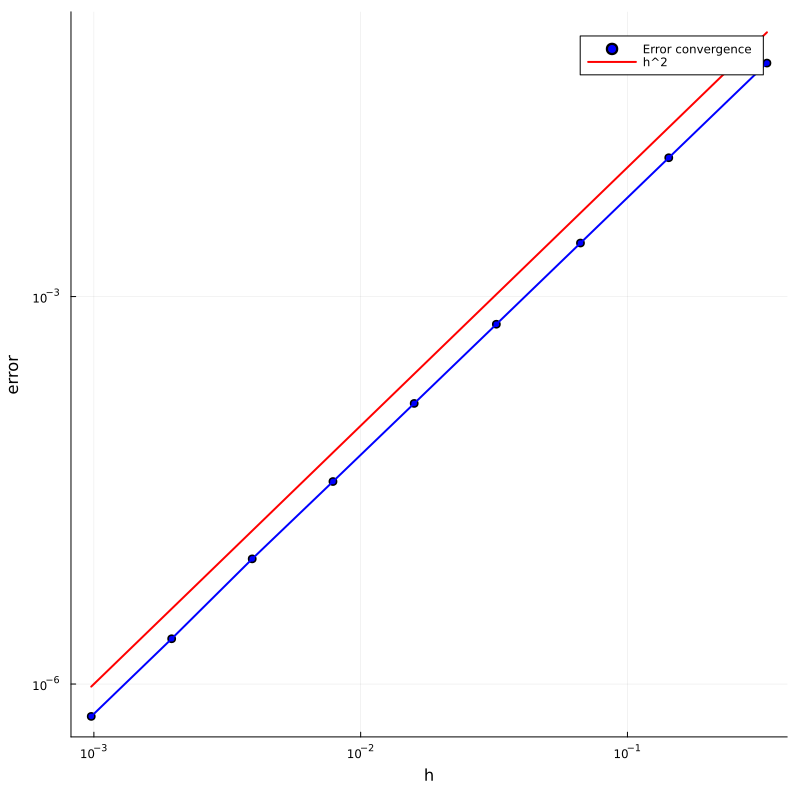
\includegraphics[width=0.85\linewidth]{errors-convergence-Gauss Seidel Tri-diagonal.png}
    \caption{Convergência do Erro do Gauss Seidel Tri-diagonal.}
  \end{figure}
\end{minipage}
\hfill
\begin{minipage}{0.45\textwidth}
  \begin{figure}[H]
    \centering
    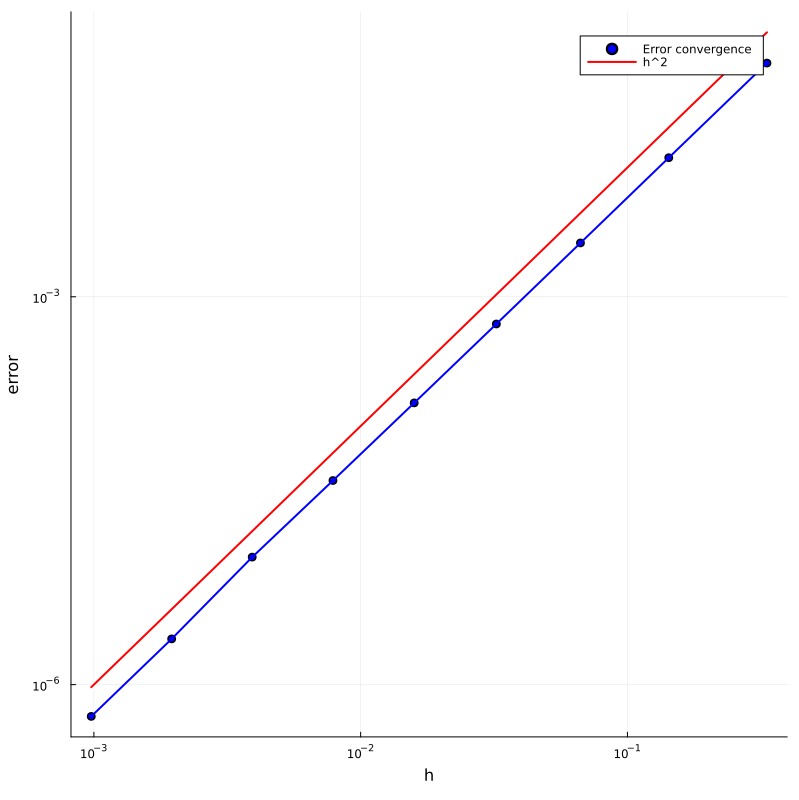
\includegraphics[width=0.85\linewidth]{errors-convergence-Gauss Jacobi Tri-diagonal.png}
    \caption{Convergência do Erro do Gauss Jacobi Tri-diagonal.}
  \end{figure}
\end{minipage}

\begin{minipage}{0.45\textwidth}
  \begin{figure}[H]
    \centering
    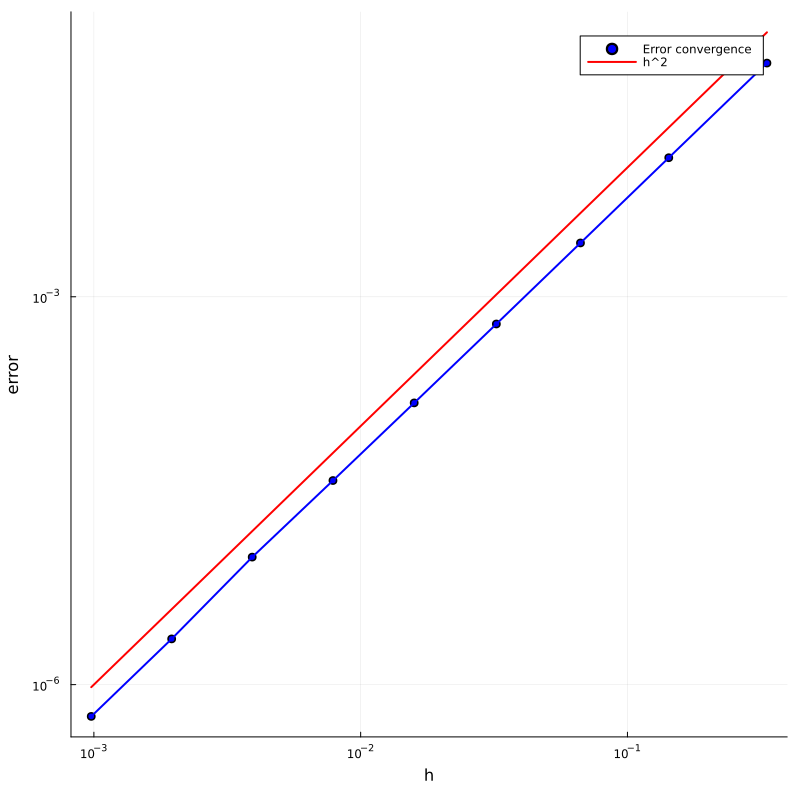
\includegraphics[width=0.85\linewidth]{errors-convergence-Gauss Jacobi Paralelo.png}
    \caption{Convergência do Erro do Gauss Jacobi Paralelo.}
  \end{figure}
\end{minipage}
\hfill
\begin{minipage}{0.45\textwidth}
  \begin{figure}[H]
    \centering
    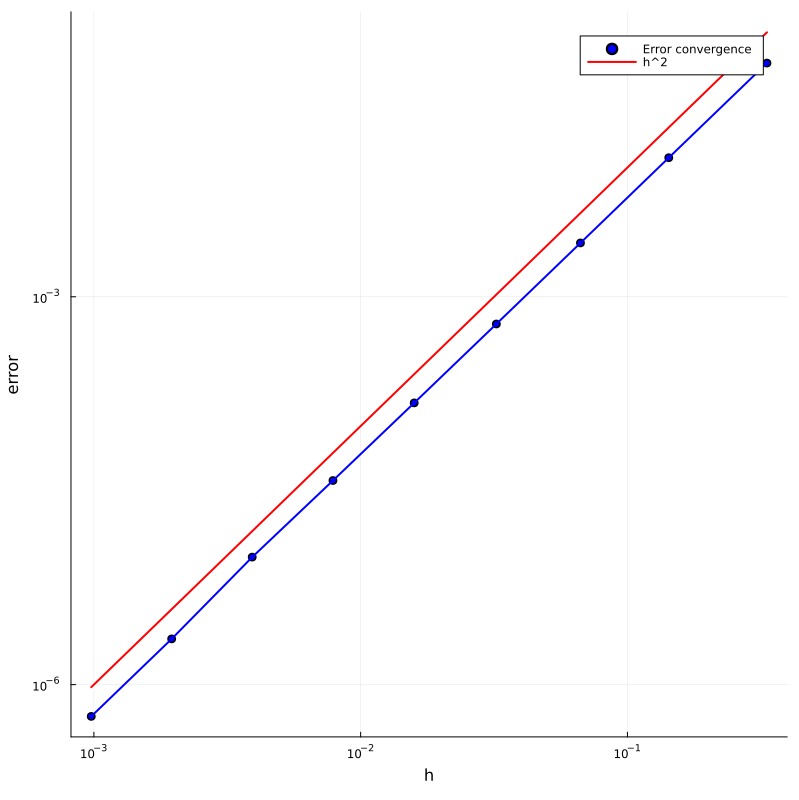
\includegraphics[width=0.85\linewidth]{errors-convergence-Gauss Jacobi Tri-diagonal Paralelo.png}
    \caption{Convergência do Erro do Gauss Jacobi Tri-diagonal Paralelo.}
  \end{figure}
\end{minipage}

Além disso, fizemos uma análise do tempo que alguns métodos iterativos e algumas de suas variações demoraram para montar as matrizes e resolver o sistema linear com o número de elementos variando em potências de 2 desde $2^2$ a $2^{10}$.

\begin{figure}[H]
  \centering
  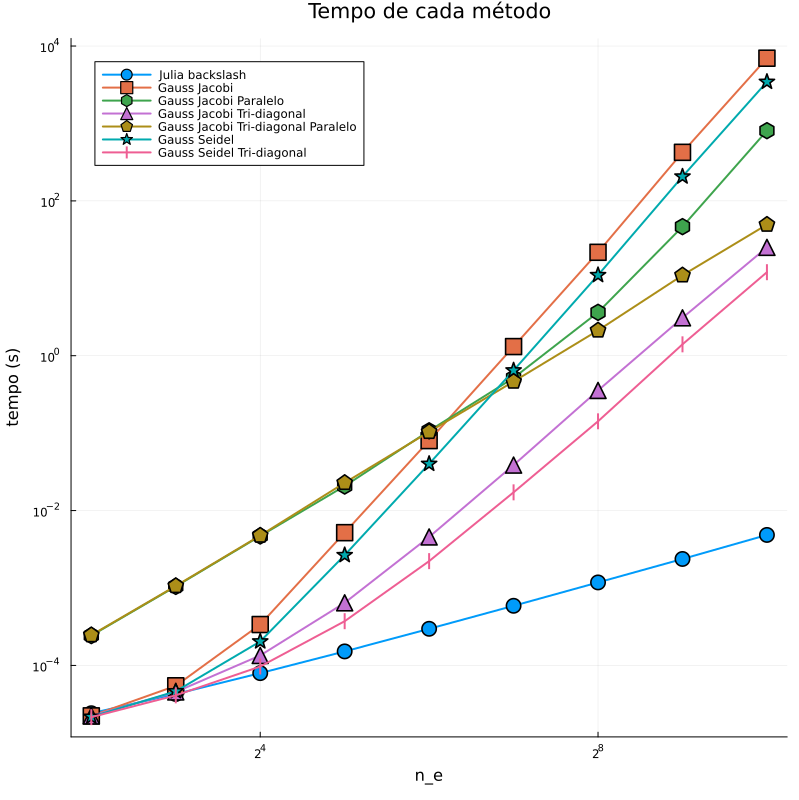
\includegraphics[width=0.85\linewidth]{compare-methods-in-solving-system-varying-ne-24-threads-2-to-10.png}
  \caption{Comparação do tempo tomado por cada método.}
\end{figure}

Para números pequenos de elementos, os métodos paralelos não se mostraram eficientes devido ao alto custo inicial do paralelismo. Entretanto, ao aumentar o número de elementos para valores superiores a $64$, o paralelismo começou a demonstrar maior viabilidade do que alguns outros métodos.

Uma análise interessante a ser feita é a inclinação de cada reta no gráfico, representada por  $\dfrac{\log_{10}(tempo)}{\log_2(ne)}$. Por exemplo, o método Gauss-Jacobi Tri-diagonal Paralelo apresenta uma inclinação menor em relação aos demais métodos, o que sugere que, para valores de $ne > 2^{10}$, ele seria a melhor escolha (desconsiderando o uso do \texttt{contra barra} do Julia). No entanto, para números pequenos de elementos, este método foi o mais lento na resolução do sistema.

Outro ponto relevante é que o gráfico utiliza escala logarítmica ($\log_{10}$) no eixo yy. Essa escala evidencia a discrepância de desempenho entre os métodos aplicados a matrizes não esparsas e os métodos otimizados. Por exemplo, o Gauss-Jacobi demorou cerca de $10^4$ segundos para resolver um sistema $1024 \times 1024$, enquanto o \texttt{contra barra} do Julia levou cerca de $10^{-3}$ segundos. Isso indica que o \texttt{contra barra} foi aproximadamente $10^7$ vezes mais rápido que o método Gauss-Jacobi.

Essa diferença de desempenho reflete o fato do \texttt{contra barra} do Julia ser um método nativo e altamente otimizado, especialmente quando combinado com a biblioteca \texttt{spzeros} utilizada nos testes. Quando aplicada a uma matriz tri-diagonal, o \texttt{contra barra} ignora as regiões não inicializadas (fora das três diagonais principais), contribuindo para seu desempenho excepcional.

Por outro lado, os métodos analisados, com exceção do \texttt{contra barra}, foram implementados manualmente, sem as otimizações típicas de métodos nativos. Isso contribui significativamente para a ineficiência observada, principalmente em matrizes de maior dimensão.